%last updated in April 2002 by Antje Endemann

\documentclass[runningheads]{llncs}
%In order to omit page numbers and running heads
%please use the following line instead of the first command line:
%\documentclass{llncs}.
%Furthermore change the line \pagestyle{headings} to
%\pagestyle{empty}.

\usepackage{graphicx, subfigure}
\usepackage{amssymb}

% Psfig/TeX 
\def\PsfigVersion{1.10}
\def\setDriver{\DvipsDriver} % \DvipsDriver or \OzTeXDriver
%
% All software, documentation, and related files in this distribution of
% psfig/tex are Copyright 1993 Trevor J. Darrell
%
% Permission is granted for use and non-profit distribution of psfig/tex 
% providing that this notice is clearly maintained. The right to
% distribute any portion of psfig/tex for profit or as part of any commercial
% product is specifically reserved for the author(s) of that portion.
%
% To use with LaTeX, use \documentstyle[psfig,...]{...}
% To use with TeX, use \input psfig.sty
%
% Bugs and improvements to trevor@media.mit.edu.
%
% Thanks to Ned Batchelder, Greg Hager (GDH), J. Daniel Smith (JDS),
% Tom Rokicki (TR), Robert Russell (RR), George V. Reilly (GVR),
% Ken McGlothlen (KHC), Baron Grey (BG), Gerhard Tobermann (GT).
% and all others who have contributed code and comments to this project!
%
% ======================================================================
% Modification History:
%
%  9 Oct 1990   JDS	used more robust bbox reading code from Tom Rokicki
% 29 Mar 1991   JDS	implemented rotation= option
% 25 Jun 1991   RR	if bb specified on cmd line don't check
%			for .ps file.
%  3 Jul 1991	JDS	check if file already read in once
%  4 Sep 1991	JDS	fixed incorrect computation of rotated
%			bounding box
% 25 Sep 1991	GVR	expanded synopsis of \psfig
% 14 Oct 1991	JDS	\fbox code from LaTeX so \psdraft works with TeX
%			changed \typeout to \ps@typeout
% 17 Oct 1991	JDS	added \psscalefirst and \psrotatefirst
% 23 Jun 1993   KHC     ``doclip'' must appear before ``rotate''
% 27 Oct 1993   TJD	removed printing of filename to avoid 
%			underscore problems. changed \frame to \fbox.
%			Added OzTeX support from BG. Added new
%			figure search path code from GT.
%
% ======================================================================
%
% Command synopsis:
%
% \psdraft	draws an outline box, but doesn't include the figure
%		in the DVI file.  Useful for previewing.
%
% \psfull	includes the figure in the DVI file (default).
%
% \psscalefirst width= or height= specifies the size of the figure
% 		before rotation.
% \psrotatefirst (default) width= or height= specifies the size of the
% 		 figure after rotation.  Asymetric figures will
% 		 appear to shrink.
%
% \psfigurepath{dir:dir:...}  sets the path to search for the figure
%
% \psfig
% usage: \psfig{file=, figure=, height=, width=,
%			bbllx=, bblly=, bburx=, bbury=,
%			rheight=, rwidth=, clip=, angle=, silent=}
%
%	"file" is the filename.  If no path name is specified and the
%		file is not found in the current directory,
%		it will be looked for in directory \psfigurepath.
%	"figure" is a synonym for "file".
%	By default, the width and height of the figure are taken from
%		the BoundingBox of the figure.
%	If "width" is specified, the figure is scaled so that it has
%		the specified width.  Its height changes proportionately.
%	If "height" is specified, the figure is scaled so that it has
%		the specified height.  Its width changes proportionately.
%	If both "width" and "height" are specified, the figure is scaled
%		anamorphically.
%	"bbllx", "bblly", "bburx", and "bbury" control the PostScript
%		BoundingBox.  If these four values are specified
%               *before* the "file" option, the PSFIG will not try to
%               open the PostScript file.
%	"rheight" and "rwidth" are the reserved height and width
%		of the figure, i.e., how big TeX actually thinks
%		the figure is.  They default to "width" and "height".
%	The "clip" option ensures that no portion of the figure will
%		appear outside its BoundingBox.  "clip=" is a switch and
%		takes no value, but the `=' must be present.
%	The "angle" option specifies the angle of rotation (degrees, ccw).
%	The "silent" option makes \psfig work silently.
%
% ======================================================================
% check to see if macros already loaded in (maybe some other file says
% "\input psfig") ...
\ifx\undefined\psfig\else\endinput\fi
%
% from a suggestion by eijkhout@csrd.uiuc.edu to allow
% loading as a style file. Changed to avoid problems
% with amstex per suggestion by jbence@math.ucla.edu

\let\LaTeXAtSign=\@
\let\@=\relax
\edef\psfigRestoreAt{\catcode`\@=\number\catcode`@\relax}
%\edef\psfigRestoreAt{\catcode`@=\number\catcode`@\relax}
\catcode`\@=11\relax
\newwrite\@unused
\def\ps@typeout#1{{\let\protect\string\immediate\write\@unused{#1}}}

\def\DvipsDriver{
	\ps@typeout{psfig/tex \PsfigVersion -dvips}
\def\PsfigSpecials{\DvipsSpecials} 	\def\ps@dir{/}
\def\ps@predir{} }
\def\OzTeXDriver{
	\ps@typeout{psfig/tex \PsfigVersion -oztex}
	\def\PsfigSpecials{\OzTeXSpecials}
	\def\ps@dir{:}
	\def\ps@predir{:}
	\catcode`\^^J=5
}

%% Here's how you define your figure path.  Should be set up with null
%% default and a user useable definition.

\def\figurepath{./:}
\def\psfigurepath#1{\edef\figurepath{#1:}}

%%% inserted for Searching Unixpaths
%%% (the path must end with :)
%%% (call: \DoPaths\figurepath )
%%%------------------------------------------------------
\def\DoPaths#1{\expandafter\EachPath#1\stoplist}
%
\def\leer{}
\def\EachPath#1:#2\stoplist{% #1 part of the list (delimiter :)
  \ExistsFile{#1}{\SearchedFile}
  \ifx#2\leer
  \else
    \expandafter\EachPath#2\stoplist
  \fi}
%
% exists the file (does not work for directories!)
%
\def\ps@dir{/}
\def\ExistsFile#1#2{%
   \openin1=\ps@predir#1\ps@dir#2
   \ifeof1
       \closein1
       %\ps@typeout{...not: \ps@predir#1\ps@dir#2}
   \else
       \closein1
       %\ps@typeout{...in:  \ps@predir#1\ps@dir#2}
        \ifx\ps@founddir\leer
          %\ps@typeout{set founddir #1}
           \edef\ps@founddir{#1}
        \fi
   \fi}
%------------------------------------------------------
%
% Get dir in path or error
%
\def\get@dir#1{%
  \def\ps@founddir{}
  \def\SearchedFile{#1}
  \DoPaths\figurepath
%  \fi
}
%------------------------------------------------------
%%% END of Searching Unixpaths


%
% @psdo control structure -- similar to Latex @for.
% I redefined these with different names so that psfig can
% be used with TeX as well as LaTeX, and so that it will not 
% be vunerable to future changes in LaTeX's internal
% control structure,
%
\def\@nnil{\@nil}
\def\@empty{}
\def\@psdonoop#1\@@#2#3{}
\def\@psdo#1:=#2\do#3{\edef\@psdotmp{#2}\ifx\@psdotmp\@empty \else
    \expandafter\@psdoloop#2,\@nil,\@nil\@@#1{#3}\fi}
\def\@psdoloop#1,#2,#3\@@#4#5{\def#4{#1}\ifx #4\@nnil \else
       #5\def#4{#2}\ifx #4\@nnil \else#5\@ipsdoloop #3\@@#4{#5}\fi\fi}
\def\@ipsdoloop#1,#2\@@#3#4{\def#3{#1}\ifx #3\@nnil 
       \let\@nextwhile=\@psdonoop \else
      #4\relax\let\@nextwhile=\@ipsdoloop\fi\@nextwhile#2\@@#3{#4}}
\def\@tpsdo#1:=#2\do#3{\xdef\@psdotmp{#2}\ifx\@psdotmp\@empty \else
    \@tpsdoloop#2\@nil\@nil\@@#1{#3}\fi}
\def\@tpsdoloop#1#2\@@#3#4{\def#3{#1}\ifx #3\@nnil 
       \let\@nextwhile=\@psdonoop \else
      #4\relax\let\@nextwhile=\@tpsdoloop\fi\@nextwhile#2\@@#3{#4}}
% 
% \fbox is defined in latex.tex; so if \fbox is undefined, assume that
% we are not in LaTeX.
% Perhaps this could be done better???
\ifx\undefined\fbox
% \fbox code from modified slightly from LaTeX
\newdimen\fboxrule
\newdimen\fboxsep
\newdimen\ps@tempdima
\newbox\ps@tempboxa
\fboxsep = 3pt
\fboxrule = .4pt
\long\def\fbox#1{\leavevmode\setbox\ps@tempboxa\hbox{#1}\ps@tempdima\fboxrule
    \advance\ps@tempdima \fboxsep \advance\ps@tempdima \dp\ps@tempboxa
   \hbox{\lower \ps@tempdima\hbox
  {\vbox{\hrule height \fboxrule
          \hbox{\vrule width \fboxrule \hskip\fboxsep
          \vbox{\vskip\fboxsep \box\ps@tempboxa\vskip\fboxsep}\hskip 
                 \fboxsep\vrule width \fboxrule}
                 \hrule height \fboxrule}}}}
\fi
%
%%%%%%%%%%%%%%%%%%%%%%%%%%%%%%%%%%%%%%%%%%%%%%%%%%%%%%%%%%%%%%%%%%%
% file reading stuff from epsf.tex
%   EPSF.TEX macro file:
%   Written by Tomas Rokicki of Radical Eye Software, 29 Mar 1989.
%   Revised by Don Knuth, 3 Jan 1990.
%   Revised by Tomas Rokicki to accept bounding boxes with no
%      space after the colon, 18 Jul 1990.
%   Portions modified/removed for use in PSFIG package by
%      J. Daniel Smith, 9 October 1990.
%
\newread\ps@stream
\newif\ifnot@eof       % continue looking for the bounding box?
\newif\if@noisy        % report what you're making?
\newif\if@atend        % %%BoundingBox: has (at end) specification
\newif\if@psfile       % does this look like a PostScript file?
%
% PostScript files should start with `%!'
%
{\catcode`\%=12\global\gdef\epsf@start{%!}}
\def\epsf@PS{PS}
%
\def\epsf@getbb#1{%
%
%   The first thing we need to do is to open the
%   PostScript file, if possible.
%
\openin\ps@stream=\ps@predir#1
\ifeof\ps@stream\ps@typeout{Error, File #1 not found}\else
%
%   Okay, we got it. Now we'll scan lines until we find one that doesn't
%   start with %. We're looking for the bounding box comment.
%
   {\not@eoftrue \chardef\other=12
    \def\do##1{\catcode`##1=\other}\dospecials \catcode`\ =10
    \loop
       \if@psfile
	  \read\ps@stream to \epsf@fileline
       \else{
	  \obeyspaces
          \read\ps@stream to \epsf@tmp\global\let\epsf@fileline\epsf@tmp}
       \fi
       \ifeof\ps@stream\not@eoffalse\else
%
%   Check the first line for `%!'.  Issue a warning message if its not
%   there, since the file might not be a PostScript file.
%
       \if@psfile\else
       \expandafter\epsf@test\epsf@fileline:. \\%
       \fi
%
%   We check to see if the first character is a % sign;
%   if so, we look further and stop only if the line begins with
%   `%%BoundingBox:' and the `(atend)' specification was not found.
%   That is, the only way to stop is when the end of file is reached,
%   or a `%%BoundingBox: llx lly urx ury' line is found.
%
          \expandafter\epsf@aux\epsf@fileline:. \\%
       \fi
   \ifnot@eof\repeat
   }\closein\ps@stream\fi}%
%
% This tests if the file we are reading looks like a PostScript file.
%
\long\def\epsf@test#1#2#3:#4\\{\def\epsf@testit{#1#2}
			\ifx\epsf@testit\epsf@start\else
\ps@typeout{Warning! File does not start with `\epsf@start'.  It may not be a PostScript file.}
			\fi
			\@psfiletrue} % don't test after 1st line
%
%   We still need to define the tricky \epsf@aux macro. This requires
%   a couple of magic constants for comparison purposes.
%
{\catcode`\%=12\global\let\epsf@percent=%\global\def\epsf@bblit{%BoundingBox}}
%
%
%   So we're ready to check for `%BoundingBox:' and to grab the
%   values if they are found.  We continue searching if `(at end)'
%   was found after the `%BoundingBox:'.
%
\long\def\epsf@aux#1#2:#3\\{\ifx#1\epsf@percent
   \def\epsf@testit{#2}\ifx\epsf@testit\epsf@bblit
	\@atendfalse
        \epsf@atend #3 . \\%
	\if@atend	
	   \if@verbose{
		\ps@typeout{psfig: found `(atend)'; continuing search}
	   }\fi
        \else
        \epsf@grab #3 . . . \\%
        \not@eoffalse
        \global\no@bbfalse
        \fi
   \fi\fi}%
%
%   Here we grab the values and stuff them in the appropriate definitions.
%
\def\epsf@grab #1 #2 #3 #4 #5\\{%
   \global\def\epsf@llx{#1}\ifx\epsf@llx\empty
      \epsf@grab #2 #3 #4 #5 .\\\else
   \global\def\epsf@lly{#2}%
   \global\def\epsf@urx{#3}\global\def\epsf@ury{#4}\fi}%
%
% Determine if the stuff following the %%BoundingBox is `(atend)'
% J. Daniel Smith.  Copied from \epsf@grab above.
%
\def\epsf@atendlit{(atend)} 
\def\epsf@atend #1 #2 #3\\{%
   \def\epsf@tmp{#1}\ifx\epsf@tmp\empty
      \epsf@atend #2 #3 .\\\else
   \ifx\epsf@tmp\epsf@atendlit\@atendtrue\fi\fi}


% End of file reading stuff from epsf.tex
%%%%%%%%%%%%%%%%%%%%%%%%%%%%%%%%%%%%%%%%%%%%%%%%%%%%%%%%%%%%%%%%%%%

%%%%%%%%%%%%%%%%%%%%%%%%%%%%%%%%%%%%%%%%%%%%%%%%%%%%%%%%%%%%%%%%%%%
% trigonometry stuff from "trig.tex"
\chardef\psletter = 11 % won't conflict with \begin{letter} now...
\chardef\other = 12

\newif \ifdebug %%% turn me on to see TeX hard at work ...
\newif\ifc@mpute %%% don't need to compute some values
\c@mputetrue % but assume that we do

\let\then = \relax
\def\r@dian{pt }
\let\r@dians = \r@dian
\let\dimensionless@nit = \r@dian
\let\dimensionless@nits = \dimensionless@nit
\def\internal@nit{sp }
\let\internal@nits = \internal@nit
\newif\ifstillc@nverging
\def \Mess@ge #1{\ifdebug \then \message {#1} \fi}

{ %%% Things that need abnormal catcodes %%%
	\catcode `\@ = \psletter
	\gdef \nodimen {\expandafter \n@dimen \the \dimen}
	\gdef \term #1 #2 #3%
	       {\edef \t@ {\the #1}%%% freeze parameter 1 (count, by value)
		\edef \t@@ {\expandafter \n@dimen \the #2\r@dian}%
				   %%% freeze parameter 2 (dimen, by value)
		\t@rm {\t@} {\t@@} {#3}%
	       }
	\gdef \t@rm #1 #2 #3%
	       {{%
		\count 0 = 0
		\dimen 0 = 1 \dimensionless@nit
		\dimen 2 = #2\relax
		\Mess@ge {Calculating term #1 of \nodimen 2}%
		\loop
		\ifnum	\count 0 < #1
		\then	\advance \count 0 by 1
			\Mess@ge {Iteration \the \count 0 \space}%
			\Multiply \dimen 0 by {\dimen 2}%
			\Mess@ge {After multiplication, term = \nodimen 0}%
			\Divide \dimen 0 by {\count 0}%
			\Mess@ge {After division, term = \nodimen 0}%
		\repeat
		\Mess@ge {Final value for term #1 of 
				\nodimen 2 \space is \nodimen 0}%
		\xdef \Term {#3 = \nodimen 0 \r@dians}%
		\aftergroup \Term
	       }}
	\catcode `\p = \other
	\catcode `\t = \other
	\gdef \n@dimen #1pt{#1} %%% throw away the ``pt''
}

\def \Divide #1by #2{\divide #1 by #2} %%% just a synonym

\def \Multiply #1by #2%%% allows division of a dimen by a dimen
       {{%%% should really freeze parameter 2 (dimen, passed by value)
	\count 0 = #1\relax
	\count 2 = #2\relax
	\count 4 = 65536
	\Mess@ge {Before scaling, count 0 = \the \count 0 \space and
			count 2 = \the \count 2}%
	\ifnum	\count 0 > 32767 %%% do our best to avoid overflow
	\then	\divide \count 0 by 4
		\divide \count 4 by 4
	\else	\ifnum	\count 0 < -32767
		\then	\divide \count 0 by 4
			\divide \count 4 by 4
		\else
		\fi
	\fi
	\ifnum	\count 2 > 32767 %%% while retaining reasonable accuracy
	\then	\divide \count 2 by 4
		\divide \count 4 by 4
	\else	\ifnum	\count 2 < -32767
		\then	\divide \count 2 by 4
			\divide \count 4 by 4
		\else
		\fi
	\fi
	\multiply \count 0 by \count 2
	\divide \count 0 by \count 4
	\xdef \product {#1 = \the \count 0 \internal@nits}%
	\aftergroup \product
       }}

\def\r@duce{\ifdim\dimen0 > 90\r@dian \then   % sin(x+90) = sin(180-x)
		\multiply\dimen0 by -1
		\advance\dimen0 by 180\r@dian
		\r@duce
	    \else \ifdim\dimen0 < -90\r@dian \then  % sin(-x) = sin(360+x)
		\advance\dimen0 by 360\r@dian
		\r@duce
		\fi
	    \fi}

\def\Sine#1%
       {{%
	\dimen 0 = #1 \r@dian
	\r@duce
	\ifdim\dimen0 = -90\r@dian \then
	   \dimen4 = -1\r@dian
	   \c@mputefalse
	\fi
	\ifdim\dimen0 = 90\r@dian \then
	   \dimen4 = 1\r@dian
	   \c@mputefalse
	\fi
	\ifdim\dimen0 = 0\r@dian \then
	   \dimen4 = 0\r@dian
	   \c@mputefalse
	\fi
%
	\ifc@mpute \then
        	% convert degrees to radians
		\divide\dimen0 by 180
		\dimen0=3.141592654\dimen0
%
		\dimen 2 = 3.1415926535897963\r@dian %%% a well-known constant
		\divide\dimen 2 by 2 %%% we only deal with -pi/2 : pi/2
		\Mess@ge {Sin: calculating Sin of \nodimen 0}%
		\count 0 = 1 %%% see power-series expansion for sine
		\dimen 2 = 1 \r@dian %%% ditto
		\dimen 4 = 0 \r@dian %%% ditto
		\loop
			\ifnum	\dimen 2 = 0 %%% then we've done
			\then	\stillc@nvergingfalse 
			\else	\stillc@nvergingtrue
			\fi
			\ifstillc@nverging %%% then calculate next term
			\then	\term {\count 0} {\dimen 0} {\dimen 2}%
				\advance \count 0 by 2
				\count 2 = \count 0
				\divide \count 2 by 2
				\ifodd	\count 2 %%% signs alternate
				\then	\advance \dimen 4 by \dimen 2
				\else	\advance \dimen 4 by -\dimen 2
				\fi
		\repeat
	\fi		
			\xdef \sine {\nodimen 4}%
       }}

% Now the Cosine can be calculated easily by calling \Sine
\def\Cosine#1{\ifx\sine\UnDefined\edef\Savesine{\relax}\else
		             \edef\Savesine{\sine}\fi
	{\dimen0=#1\r@dian\advance\dimen0 by 90\r@dian
	 \Sine{\nodimen 0}
	 \xdef\cosine{\sine}
	 \xdef\sine{\Savesine}}}	      
% end of trig stuff
%%%%%%%%%%%%%%%%%%%%%%%%%%%%%%%%%%%%%%%%%%%%%%%%%%%%%%%%%%%%%%%%%%%%

\def\psdraft{
	\def\@psdraft{0}
	%\ps@typeout{draft level now is \@psdraft \space . }
}
\def\psfull{
	\def\@psdraft{100}
	%\ps@typeout{draft level now is \@psdraft \space . }
}

\psfull

\newif\if@scalefirst
\def\psscalefirst{\@scalefirsttrue}
\def\psrotatefirst{\@scalefirstfalse}
\psrotatefirst

\newif\if@draftbox
\def\psnodraftbox{
	\@draftboxfalse
}
\def\psdraftbox{
	\@draftboxtrue
}
\@draftboxtrue

\newif\if@prologfile
\newif\if@postlogfile
\def\pssilent{
	\@noisyfalse
}
\def\psnoisy{
	\@noisytrue
}
\psnoisy
%%% These are for the option list.
%%% A specification of the form a = b maps to calling \@p@@sa{b}
\newif\if@bbllx
\newif\if@bblly
\newif\if@bburx
\newif\if@bbury
\newif\if@height
\newif\if@width
\newif\if@rheight
\newif\if@rwidth
\newif\if@angle
\newif\if@clip
\newif\if@verbose
\def\@p@@sclip#1{\@cliptrue}
%
%
\newif\if@decmpr
%
\def\@p@@sfigure#1{\def\@p@sfile{null}\def\@p@sbbfile{null}\@decmprfalse
   % look directly for file (e.g. absolute path)
   \openin1=\ps@predir#1
   \ifeof1
	\closein1
	% failed, search directories for file
	\get@dir{#1}
	\ifx\ps@founddir\leer
		% failed, search directly for file.bb
		\openin1=\ps@predir#1.bb
		\ifeof1
			\closein1
			% failed, search directories for file.bb
			\get@dir{#1.bb}
			\ifx\ps@founddir\leer
				% failed, lose.
				\ps@typeout{Can't find #1 in \figurepath}
			\else
				% found file.bb in search dir
				\@decmprtrue
				\def\@p@sfile{\ps@founddir\ps@dir#1}
				\def\@p@sbbfile{\ps@founddir\ps@dir#1.bb}
			\fi
		\else
			\closein1
			%found file.bb directly
			\@decmprtrue
			\def\@p@sfile{#1}
			\def\@p@sbbfile{#1.bb}
		\fi
	\else
		% found file in search dir
		\def\@p@sfile{\ps@founddir\ps@dir#1}
		\def\@p@sbbfile{\ps@founddir\ps@dir#1}
	\fi
   \else
	% found file directly
	\closein1
	\def\@p@sfile{#1}
	\def\@p@sbbfile{#1}
   \fi
}
%
%
%
\def\@p@@sfile#1{\@p@@sfigure{#1}}
%
\def\@p@@sbbllx#1{
		%\ps@typeout{bbllx is #1}
		\@bbllxtrue
		\dimen100=#1
		\edef\@p@sbbllx{\number\dimen100}
}
\def\@p@@sbblly#1{
		%\ps@typeout{bblly is #1}
		\@bbllytrue
		\dimen100=#1
		\edef\@p@sbblly{\number\dimen100}
}
\def\@p@@sbburx#1{
		%\ps@typeout{bburx is #1}
		\@bburxtrue
		\dimen100=#1
		\edef\@p@sbburx{\number\dimen100}
}
\def\@p@@sbbury#1{
		%\ps@typeout{bbury is #1}
		\@bburytrue
		\dimen100=#1
		\edef\@p@sbbury{\number\dimen100}
}
\def\@p@@sheight#1{
		\@heighttrue
		\dimen100=#1
   		\edef\@p@sheight{\number\dimen100}
		%\ps@typeout{Height is \@p@sheight}
}
\def\@p@@swidth#1{
		%\ps@typeout{Width is #1}
		\@widthtrue
		\dimen100=#1
		\edef\@p@swidth{\number\dimen100}
}
\def\@p@@srheight#1{
		%\ps@typeout{Reserved height is #1}
		\@rheighttrue
		\dimen100=#1
		\edef\@p@srheight{\number\dimen100}
}
\def\@p@@srwidth#1{
		%\ps@typeout{Reserved width is #1}
		\@rwidthtrue
		\dimen100=#1
		\edef\@p@srwidth{\number\dimen100}
}
\def\@p@@sangle#1{
		%\ps@typeout{Rotation is #1}
		\@angletrue
%		\dimen100=#1
		\edef\@p@sangle{#1} %\number\dimen100}
}
\def\@p@@ssilent#1{ 
		\@verbosefalse
}
\def\@p@@sprolog#1{\@prologfiletrue\def\@prologfileval{#1}}
\def\@p@@spostlog#1{\@postlogfiletrue\def\@postlogfileval{#1}}
\def\@cs@name#1{\csname #1\endcsname}
\def\@setparms#1=#2,{\@cs@name{@p@@s#1}{#2}}
%
% initialize the defaults (size the size of the figure)
%
\def\ps@init@parms{
		\@bbllxfalse \@bbllyfalse
		\@bburxfalse \@bburyfalse
		\@heightfalse \@widthfalse
		\@rheightfalse \@rwidthfalse
		\def\@p@sbbllx{}\def\@p@sbblly{}
		\def\@p@sbburx{}\def\@p@sbbury{}
		\def\@p@sheight{}\def\@p@swidth{}
		\def\@p@srheight{}\def\@p@srwidth{}
		\def\@p@sangle{0}
		\def\@p@sfile{} \def\@p@sbbfile{}
		\def\@p@scost{10}
		\def\@sc{}
		\@prologfilefalse
		\@postlogfilefalse
		\@clipfalse
		\if@noisy
			\@verbosetrue
		\else
			\@verbosefalse
		\fi
}
%
% Go through the options setting things up.
%
\def\parse@ps@parms#1{
	 	\@psdo\@psfiga:=#1\do
		   {\expandafter\@setparms\@psfiga,}}
%
% Compute bb height and width
%
\newif\ifno@bb
\def\bb@missing{
	\if@verbose{
		\ps@typeout{psfig: searching \@p@sbbfile \space  for bounding box}
	}\fi
	\no@bbtrue
	\epsf@getbb{\@p@sbbfile}
        \ifno@bb \else \bb@cull\epsf@llx\epsf@lly\epsf@urx\epsf@ury\fi
}	
\def\bb@cull#1#2#3#4{
	\dimen100=#1 bp\edef\@p@sbbllx{\number\dimen100}
	\dimen100=#2 bp\edef\@p@sbblly{\number\dimen100}
	\dimen100=#3 bp\edef\@p@sbburx{\number\dimen100}
	\dimen100=#4 bp\edef\@p@sbbury{\number\dimen100}
	\no@bbfalse
}
% rotate point (#1,#2) about (0,0).
% The sine and cosine of the angle are already stored in \sine and
% \cosine.  The result is placed in (\p@intvaluex, \p@intvaluey).
\newdimen\p@intvaluex
\newdimen\p@intvaluey
\def\rotate@#1#2{{\dimen0=#1 sp\dimen1=#2 sp
%            	calculate x' = x \cos\theta - y \sin\theta
		  \global\p@intvaluex=\cosine\dimen0
		  \dimen3=\sine\dimen1
		  \global\advance\p@intvaluex by -\dimen3
% 		calculate y' = x \sin\theta + y \cos\theta
		  \global\p@intvaluey=\sine\dimen0
		  \dimen3=\cosine\dimen1
		  \global\advance\p@intvaluey by \dimen3
		  }}
\def\compute@bb{
		\no@bbfalse
		\if@bbllx \else \no@bbtrue \fi
		\if@bblly \else \no@bbtrue \fi
		\if@bburx \else \no@bbtrue \fi
		\if@bbury \else \no@bbtrue \fi
		\ifno@bb \bb@missing \fi
		\ifno@bb \ps@typeout{FATAL ERROR: no bb supplied or found}
			\no-bb-error
		\fi
		%
%\ps@typeout{BB: \@p@sbbllx, \@p@sbblly, \@p@sbburx, \@p@sbbury} 
%
% store height/width of original (unrotated) bounding box
		\count203=\@p@sbburx
		\count204=\@p@sbbury
		\advance\count203 by -\@p@sbbllx
		\advance\count204 by -\@p@sbblly
		\edef\ps@bbw{\number\count203}
		\edef\ps@bbh{\number\count204}
		%\ps@typeout{ psbbh = \ps@bbh, psbbw = \ps@bbw }
		\if@angle 
			\Sine{\@p@sangle}\Cosine{\@p@sangle}
	        	{\dimen100=\maxdimen\xdef\r@p@sbbllx{\number\dimen100}
					    \xdef\r@p@sbblly{\number\dimen100}
			                    \xdef\r@p@sbburx{-\number\dimen100}
					    \xdef\r@p@sbbury{-\number\dimen100}}
%
% Need to rotate all four points and take the X-Y extremes of the new
% points as the new bounding box.
                        \def\minmaxtest{
			   \ifnum\number\p@intvaluex<\r@p@sbbllx
			      \xdef\r@p@sbbllx{\number\p@intvaluex}\fi
			   \ifnum\number\p@intvaluex>\r@p@sbburx
			      \xdef\r@p@sbburx{\number\p@intvaluex}\fi
			   \ifnum\number\p@intvaluey<\r@p@sbblly
			      \xdef\r@p@sbblly{\number\p@intvaluey}\fi
			   \ifnum\number\p@intvaluey>\r@p@sbbury
			      \xdef\r@p@sbbury{\number\p@intvaluey}\fi
			   }
%			lower left
			\rotate@{\@p@sbbllx}{\@p@sbblly}
			\minmaxtest
%			upper left
			\rotate@{\@p@sbbllx}{\@p@sbbury}
			\minmaxtest
%			lower right
			\rotate@{\@p@sbburx}{\@p@sbblly}
			\minmaxtest
%			upper right
			\rotate@{\@p@sbburx}{\@p@sbbury}
			\minmaxtest
			\edef\@p@sbbllx{\r@p@sbbllx}\edef\@p@sbblly{\r@p@sbblly}
			\edef\@p@sbburx{\r@p@sbburx}\edef\@p@sbbury{\r@p@sbbury}
%\ps@typeout{rotated BB: \r@p@sbbllx, \r@p@sbblly, \r@p@sbburx, \r@p@sbbury}
		\fi
		\count203=\@p@sbburx
		\count204=\@p@sbbury
		\advance\count203 by -\@p@sbbllx
		\advance\count204 by -\@p@sbblly
		\edef\@bbw{\number\count203}
		\edef\@bbh{\number\count204}
		%\ps@typeout{ bbh = \@bbh, bbw = \@bbw }
}
%
% \in@hundreds performs #1 * (#2 / #3) correct to the hundreds,
%	then leaves the result in @result
%
\def\in@hundreds#1#2#3{\count240=#2 \count241=#3
		     \count100=\count240	% 100 is first digit #2/#3
		     \divide\count100 by \count241
		     \count101=\count100
		     \multiply\count101 by \count241
		     \advance\count240 by -\count101
		     \multiply\count240 by 10
		     \count101=\count240	%101 is second digit of #2/#3
		     \divide\count101 by \count241
		     \count102=\count101
		     \multiply\count102 by \count241
		     \advance\count240 by -\count102
		     \multiply\count240 by 10
		     \count102=\count240	% 102 is the third digit
		     \divide\count102 by \count241
		     \count200=#1\count205=0
		     \count201=\count200
			\multiply\count201 by \count100
		 	\advance\count205 by \count201
		     \count201=\count200
			\divide\count201 by 10
			\multiply\count201 by \count101
			\advance\count205 by \count201
			%
		     \count201=\count200
			\divide\count201 by 100
			\multiply\count201 by \count102
			\advance\count205 by \count201
			%
		     \edef\@result{\number\count205}
}
\def\compute@wfromh{
		% computing : width = height * (bbw / bbh)
		\in@hundreds{\@p@sheight}{\@bbw}{\@bbh}
		%\ps@typeout{ \@p@sheight * \@bbw / \@bbh, = \@result }
		\edef\@p@swidth{\@result}
		%\ps@typeout{w from h: width is \@p@swidth}
}
\def\compute@hfromw{
		% computing : height = width * (bbh / bbw)
	        \in@hundreds{\@p@swidth}{\@bbh}{\@bbw}
		%\ps@typeout{ \@p@swidth * \@bbh / \@bbw = \@result }
		\edef\@p@sheight{\@result}
		%\ps@typeout{h from w : height is \@p@sheight}
}
\def\compute@handw{
		\if@height 
			\if@width
			\else
				\compute@wfromh
			\fi
		\else 
			\if@width
				\compute@hfromw
			\else
				\edef\@p@sheight{\@bbh}
				\edef\@p@swidth{\@bbw}
			\fi
		\fi
}
\def\compute@resv{
		\if@rheight \else \edef\@p@srheight{\@p@sheight} \fi
		\if@rwidth \else \edef\@p@srwidth{\@p@swidth} \fi
		%\ps@typeout{rheight = \@p@srheight, rwidth = \@p@srwidth}
}
%		
% Compute any missing values
\def\compute@sizes{
	\compute@bb
	\if@scalefirst\if@angle
% at this point the bounding box has been adjsuted correctly for
% rotation.  PSFIG does all of its scaling using \@bbh and \@bbw.  If
% a width= or height= was specified along with \psscalefirst, then the
% width=/height= value needs to be adjusted to match the new (rotated)
% bounding box size (specifed in \@bbw and \@bbh).
%    \ps@bbw       width=
%    -------  =  ---------- 
%    \@bbw       new width=
% so `new width=' = (width= * \@bbw) / \ps@bbw; where \ps@bbw is the
% width of the original (unrotated) bounding box.
	\if@width
	   \in@hundreds{\@p@swidth}{\@bbw}{\ps@bbw}
	   \edef\@p@swidth{\@result}
	\fi
	\if@height
	   \in@hundreds{\@p@sheight}{\@bbh}{\ps@bbh}
	   \edef\@p@sheight{\@result}
	\fi
	\fi\fi
	\compute@handw
	\compute@resv}
%
%
%
\def\OzTeXSpecials{
	\special{empty.ps /@isp {true} def}
	\special{empty.ps \@p@swidth \space \@p@sheight \space
			\@p@sbbllx \space \@p@sbblly \space
			\@p@sbburx \space \@p@sbbury \space
			startTexFig \space }
	\if@clip{
		\if@verbose{
			\ps@typeout{(clip)}
		}\fi
		\special{empty.ps doclip \space }
	}\fi
	\if@angle{
		\if@verbose{
			\ps@typeout{(rotate)}
		}\fi
		\special {empty.ps \@p@sangle \space rotate \space} 
	}\fi
	\if@prologfile
	    \special{\@prologfileval \space } \fi
	\if@decmpr{
		\if@verbose{
			\ps@typeout{psfig: Compression not available
			in OzTeX version \space }
		}\fi
	}\else{
		\if@verbose{
			\ps@typeout{psfig: including \@p@sfile \space }
		}\fi
		\special{epsf=\@p@sfile \space }
	}\fi
	\if@postlogfile
	    \special{\@postlogfileval \space } \fi
	\special{empty.ps /@isp {false} def}
}
\def\DvipsSpecials{
	%
	\special{ps::[begin] 	\@p@swidth \space \@p@sheight \space
			\@p@sbbllx \space \@p@sbblly \space
			\@p@sbburx \space \@p@sbbury \space
			startTexFig \space }
	\if@clip{
		\if@verbose{
			\ps@typeout{(clip)}
		}\fi
		\special{ps:: doclip \space }
	}\fi
	\if@angle
		\if@verbose{
			\ps@typeout{(clip)}
		}\fi
		\special {ps:: \@p@sangle \space rotate \space} 
	\fi
	\if@prologfile
	    \special{ps: plotfile \@prologfileval \space } \fi
	\if@decmpr{
		\if@verbose{
			\ps@typeout{psfig: including \@p@sfile.Z \space }
		}\fi
		\special{ps: plotfile "`zcat \@p@sfile.Z" \space }
	}\else{
		\if@verbose{
			\ps@typeout{psfig: including \@p@sfile \space }
		}\fi
		\special{ps: plotfile \@p@sfile \space }
	}\fi
	\if@postlogfile
	    \special{ps: plotfile \@postlogfileval \space } \fi
	\special{ps::[end] endTexFig \space }
}
%
% \psfig
% usage : \psfig{file=, height=, width=, bbllx=, bblly=, bburx=, bbury=,
%			rheight=, rwidth=, clip=}
%
% "clip=" is a switch and takes no value, but the `=' must be present.
\def\psfig#1{\vbox {
	% do a zero width hard space so that a single
	% \psfig in a centering enviornment will behave nicely
	%{\setbox0=\hbox{\ }\ \hskip-\wd0}
	%
	\ps@init@parms
	\parse@ps@parms{#1}
	\compute@sizes
	%
	\ifnum\@p@scost<\@psdraft{
		\PsfigSpecials 
		% Create the vbox to reserve the space for the figure.
		\vbox to \@p@srheight sp{
		% 1/92 TJD Changed from "true sp" to "sp" for magnification.
			\hbox to \@p@srwidth sp{
				\hss
			}
		\vss
		}
	}\else{
		% draft figure, just reserve the space and print the
		% path name.
		\if@draftbox{		
			% Verbose draft: print file name in box
			% 10/93 TJD changed to fbox from frame
			\hbox{\fbox{\vbox to \@p@srheight sp{
			\vss
			\hbox to \@p@srwidth sp{ \hss 
			        % 10/93 TJD deleted to avoid ``_'' problems
				% \@p@sfile
			 \hss }
			\vss
			}}}
		}\else{
			% Non-verbose draft
			\vbox to \@p@srheight sp{
			\vss
			\hbox to \@p@srwidth sp{\hss}
			\vss
			}
		}\fi	



	}\fi
}}
\psfigRestoreAt
\setDriver
\let\@=\LaTeXAtSign





\begin{document}

\pagestyle{headings}
%In order to omit page numbers and running heads
%please change this line to
%\pagestyle{empty}
%and change the first command line too, see above.

\author{Christopher J. Gibson\thanks{e-mail: cgibson@calpoly.edu}
\and Zo\"{e} J. Wood\thanks{e-mail: zwood@calpoly.edu}}

\institute{California Polytechnic State University}

\mainmatter

\title{An Approach to Point Based Approximate Color Bleeding With Volumes}

\titlerunning{Point Based Color Bleeding With Volumes}

\maketitle


\begin{abstract}
Achieving realistic or believable global illumination in scenes with participating media is expensive.  Light interacts with the particles of a volume, creating complex radiance patterns.  This paper introduces an explicit extension to the commonly used point-based color bleeding technique which allows fast, believable in- and out-scattering effects building on existing data structures and paradigms.  The proposed method achieves results comparable to that of existing Monte Carlo integration methods, that is realistic looking renders of scenes which include volume data elements, obtaining render speeds between 10 and 36 times faster while keeping memory overhead under 5\%.
\end{abstract}



%==============================================================================%
\section{Introduction}
The ability to render scenes with realistic lighting is desirable for many entertainment application settings such as film.  Great results have been achieved for large scenes using point based color bleeding~\cite{christensen:2008} algorithms.  In their basic form, these algorithms tend to limit or omit the lighting contribution from volumetric data or participating media within the scenes.  This paper presents an explicit extension to the point-based color bleeding (PCB) algorithm and data representation tuned to volumes,  \emph{light-voxel (or lvoxel)} to address the need to represent participating media which leverages a point cloud representation of a scene.  

  The proposed method achieves results comparable to those produced with Monte Carlo ray tracing~\cite{MCRay1}, that is, images that include color bleeding from volume elements but with drastically reduced run times, speeding up renders by around 10 to 36 times.  Figure~\ref{fig:compare1} illustrates a comparison of our algorithm and Monte Carlo ray traced results.


\subsection{Background}
\label{background_sec}
The goal of the proposed method is to include volumetric representations into a global illumination algorithm in a fast and coherent way. One of the unique features of participating media is that they must be represented with a more complex data-structure than solid geometric objects which are usually polygonalized in most rendering processes.  Light interacts with the particles of a volume, creating complex radiance patterns (increasing the necessary computational complexity exponentially.) In particular the most fundamental concepts are presented here,  (based off of  \cite{pbrt}).

In contrast to polygonal models, in volumes, as light passes through a participating media, light will: become absorbed based on its absorption probability density $\sigma_{a}$ and light can be scattered based on a scatter probability density $\sigma_{s}$.  Both \emph{absorption} and \emph{scatter-out} involve the reduction of energy through a volume, reducing its transmittance, which can be combined into the following representation: $\sigma_{t}(\textup{p},w) = \sigma_{a}(\textup{p},w) + \sigma_{s}(\textup{p}, w)$.
Then, integrating the transmittion of the volume over a ray gives us equation (1.1): $T_{r}(\textup{p} \to \textup{p}') = e^{-\int_{0}^{d}\sigma_{t} (p+t\mathit{w},\mathit{w})d\mathit{t}}\label{transmittion_eq}$.

Additionally, in volumes, the probability that light may scatter from direction $w$ to $w'$ is described using a distribution function or \textit{phase function}, which describes the angular distribution of light scattered by particles in a volume.  All tests in this paper were rendered using one of the simplest phase functions, known as the isotropic or \textit{constant} phase function which represents the BRDF analog for participating media~\cite{cerezo}.

Finally, while $\sigma_{s}$ may reduce the energy of a ray passing through a volume, radiance from other rays may contribute to the original ray's radiance, called \emph{scatter-in}.  After we guarantee that the distribution is normalized,  to make sure that the phase function actually defines a proper probability distribution for a particular direction, we can integrate the total radiance scatter based on the normalized phase function $phase(w \to w')$ over all directions $w'$ to get our total scatter in a direction $w$: $\mathit{S}(\textup{p},w) = \mathit{L}_{\textup{ve}}(\textup{p},w) + \sigma_{\textup{s}}(\textup{p}, w) \int_{\mathbb{S}^2} phase(\textup{p}, -w' \to w) L_{i}(\textup{p},w')\textup{d}w'.$  The volume emission coefficient, $L_{\textup{ve}}(\textup{p}, w)$, is not discussed here.


\section{Related Work}

\paragraph{Global Illumination:}
Global illumination is an important problem in computer graphics, with numerous successful algorithmic solutions, including, photon mapping \cite{Jensen:2009}, radiosity \cite{radiosity} and Monte Carlo sampling techniques for ray tracing~\cite{MCRay1}.  The most closely related methods to this work are those that sample the scene and use a two stage approach to model direct and indirect illumination. Of particular relevance is Point-Based Approximate Color Bleeding \cite{christensen:2008}, which describes the process of sampling the scene in order to create a point cloud representation, used to evaluate the incoming radiance surrounding a given point on a surface.  As recently as 2010, discussion of approximating volume scattering using point clouds was mentioned in \cite{christensen:siggraph}, but without algorithmic details, such as how \textit{back-to-front or front-to-back rasterization} would be achieved with the current rasterization method (handled by our octree traversal method) or how scatter, extinction and absorption would be managed within the volume representation in the point cloud.

Other closely related work includes attempts at simulating light scatter and absorption properties of participating media through existing photon mapping techniques, which have shown promise in the past.  Jensen in~\cite{jensen:1998} describes a process where photons participate and become stored inside the volume itself for later gathers during volume integration.  While this technique is shown to work, it primarily focuses on caustic effects in volumes and the generated photon map.  Our storage method does not require data to be stored in the volume, but in a separate, more lightweight data-structure better suited for out-of-core rendering.

\paragraph{Volume Rendering:}
This paper is focused on the rendering of scenes which contain volume data.  A number of approaches have been developed in order to render volume data~\cite{levoy88}\cite{Kajiya84}.  Volume data representations often include an efficient multi-resolution data representation~\cite{Westermann94}\cite{Levoy90}.  When dealing with multi-resolution volume octree datastructures, removing occluded nodes from being tested can drastically increase performance \cite{guthe}.  Our algorithm takes advantage of a multi-resolution, view-independant octree datastructure in order to handle a large amount of complex lighting and volume data, skipping material occluded by opaque geometry cached in the data-structure in the form of surfels.  Although the idea of using these techniques in volumes is not new, utilizing them to guarentee correct volume integration in the point cloud used in PCB is.
% a new development, which will be described in more detail in Section \ref{scatterout_sec}.

%==============================================================================%
\section{Algorithm}
\label{algorithm_sec}
We present an algorithm which is an extension to the point cloud techniques described in \cite{tabellion} and \cite{christensen:2008}, specifically building off the point-based color bleeding technique by Christensen.  The modifications involve evaluating light scatter and absorption properties at discrete points in the volume and adding them to the point cloud.  Using a front-to-back traversal method, we can correctly and quickly approximate the \textit{light-volume} representation's contribution to a scene's indirect lighting evaluation.

In general, PCB methods subdivide the world into small representational segments, called surfels~\cite{christensen:2008}, which are stored in a large point cloud, representing the scene.  Surfels are used to model direct illumination, and are then used in a later phase to compute indirect lighting and color bleeding in an efficient manner.  

The goal of our method is to include volumetric representations into PCB methods in a fast and coherent way while keeping memory overhead and computational complexity to a minimum.  In the existing algorithms~\cite{christensen:2008}, surfels represent opaque materials within the point cloud, thus to incorporate a representation of volumetric data, an additional data representation was necessary to handle the scatter and absorption properties of participating media.  Our data representation closely follows the model of surfels, in that we choose to sample the volume at discrete locations and store a finite representation of the lighting at those discrete locations, but with modifications to handle the special attributes of lighting in transparent media.  In keeping with the naming conventions established, we call our discrete sampling of lighting elements for a volume: \emph{lvoxels}.  

In general, our algorithm must 1) sample the scene geometry (including the volume) and store the direct lighting (or relevant lighting properties) 2) gather indirect lighting and 3) model the scatter-out and scatter-in properties of volumetric lighting.

\subsection{Sampling the Scene}
The goal of this stage of the algorithm is to sample the scene geometry (including the volume) and store the direct lighting in a finite data representation to be used later for global illumination lighting effects.  As all of our finite data represents the direct lighting of some small portion of a surface or element in a three-dimensional scene, we refer to the union of all finite lighting samples as a ``point cloud''.  This point cloud is stored in an octree representation for efficient access to all data elements, surfels and lvoxels.  Surfels differ from lvoxels only in that surfels represent a flat, solid geometry while lvoxels represent a transparent, volumetric medium.  Both have radii and position so both can be placed within the same point cloud.  

We sample the opaque geometry as surfels, which are computed using a perspective viewing volume slightly larger then the current viewing frustum, with a sampling rate two times that of the desired pixel resolution.  Rays are cast from this logical camera just as we would ray trace a normal scene, with surfels generated where those rays intersect with the scene.  Lvoxels are generated by marching over the entire domain of the volume by a specific, preset interval, sampling scatter and absorption coefficients in order to get an average throughout the area an lvoxel will occupy.  Typically this involves eight to sixteen absorption and scatter samples per lvoxel.  These values, as well as the radius of the lvoxels, may differ depending on the complexity and raw resolution of the volume.  In our tests, one lvoxel for every $2^3 - 4^3$ voxels achieved good results.

Caching the direct light contribution at each lvoxel by testing the transmittance (equation \ref{transmittion_eq}) to each light source saves us from re-computing light calculations during sampling in sections \ref{scatterout_sec} and \ref{scatterin_sec} \cite{signotes:2010}.


\subsection{Gathering Light}
\label{gather_sec}

Next, our algorithm uses a gather stage similar to the one in PCB, which calculates the irradiance at a point on a surface, given the radiance of the scene around it.  Unlike PCB, which uses a software rasterization method, we chose to evaluate irradiance by raycasting into the point-cloud around a hemisphere oriented along the surface's normal.  This decision was made to simplify the tests which compare traditional Monte Carlo sampling methods to the extended PCB algorithm, but also to simplify evaluation of the transparent lvoxels.

In order to approximate the integral of incoming light at point $p$ on the surface, we sample across a hemisphere oriented along the surface's normal $N$ at $\textup{p}$.  Each sample cast out from $p$ evaluates $L(\textup{p} \leftarrow w)$ which is then multiplied by $w \cdot N$ in order to represent $cos\theta$.  In order to obtain good results, 128-256 samples are typically necessary to combat noise caused by the samples.  How radiance and transmittance are handled with lvoxels will be explained in the next section.


%------------------------------------------------------------%
\subsection{Adding Scatter-Out}
\label{scatterout_sec}
Modifications to the previously mentioned irradiance sampling technique for scatter-out effects with volumes are few.  The most significant changes are to the point cloud octree and its traversal.  Specifically, when computing lighting, we must account for the fact that when an element of the point cloud is hit, it may be transparent.  In the standard algorithm, absorption and transmittance would not be taken into account and the traversal would stop at the first lvoxel encountered.

In order to properly evaluate transparent and opaque surfaces within the point cloud, we made changes to node-level octree traversal.  Each branch traverses its children from closest to farthest, guaranteeing that closer leaf nodes are evaluated first.  Leaf nodes then use the pre-evaluated scatter ($\sigma_{s}$) and absorption ($\sigma_{t}$) coefficients for each lvoxel to appropriately alter the sample ray's transmittance, and continue with the traversal, with each hit contributing to the final resulting radiance value.  Once a surfel is hit, there is no need to continue traversing the octree.

In addition to traversing the tree front-to-back, we also keep track of the incoming radiance and current transmittance.  Both of these values are modified according to the equations described in Section \ref{background_sec} taking into account each lvoxel's scatter and absorption coefficients.


%------------------------------------------------------------%
\subsection{Adding Scatter-In}
\label{scatterin_sec}
After adding lvoxels to our octree structure and evaluation algorithm, the only modifications necessary for scatter-in are to the volume rendering equation.  Recall that to model lighting for a volume, in-scattering requires integrating over all directions.  Casting Monte Carlo sample rays through the volume and into the scene would be computationally expensive.  Instead, for each sample we send out rays into the point cloud, iterating through a much sparser dataset.  This helps us replace expensive $S(\textup{p, w})$ evaluations with traversals into the octree.  The two main differences between sampling scattered light within a volume and evaluating the irradiance on a surface are 1) the distribution function, which is based on the volume's phase function, and 2) the samples are distributed over a sphere rather than a hemisphere.  Each of these samples gather light as described in Section \ref{gather_sec}.


%==============================================================================%
\section{Results}
Our algorithm is able to achieve realistic lighting effects for scenes that include volumetric elements using our lvoxel representation with a point-based color bleeding approach to global illumination.
All test cases were run on a commodity-class Intel i5 3 GHz machine with 4 Gb of RAM.  Because of the disparity between academic-level versus production-class ray tracer implementations, we tested and compared our results against a naive implementation of Monte Carlo global illumination not using the point cloud representation.  We then compared the resulting images and render times of each.  Our algorithm is able to achieve a very small image difference and an increase in render time efficiency.

The scene tested involved a 60,000 triangle Sponza Atrium model including only vertex and normal information for simplicity.  CT scan datasets of a human head and the Stanford Bunny were used in order to test scatter in/out contributions by complex participating media.
Both Figures~\ref{fig:compare1} and~\ref{fig:compare2} show the CT data in Sponza Atrium rendered with traditional Monte Carlo scattering and our extended PCB.  These resulting renders are very similar, and a closer look in Figure~\ref{fig:compare_second}, exemplifies the great similarity between the two images.  However, there are some small artifacts present in the image rendered with the point cloud representation, and the indirect lighting is slightly darker overall. 

\begin{figure}[]
    \centering
    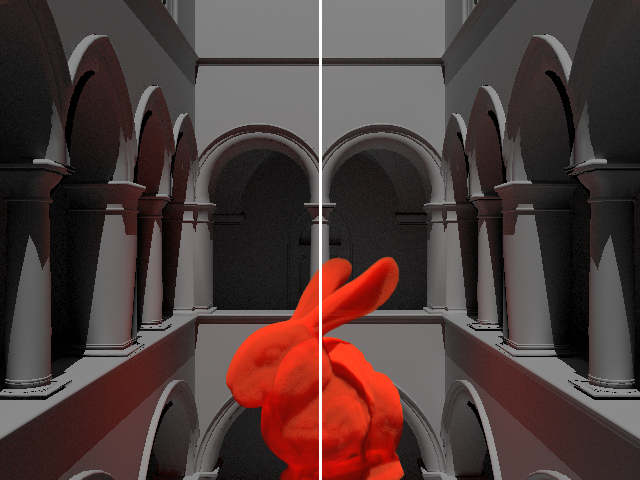
\includegraphics[width=90mm]{img/compare.png}
    \caption{Bunny Scene comparison of the PCB extension (left) and traditional Monte Carlo results (right.)}
    \label{fig:compare1}
\end{figure}


\begin{figure}
    \centering
    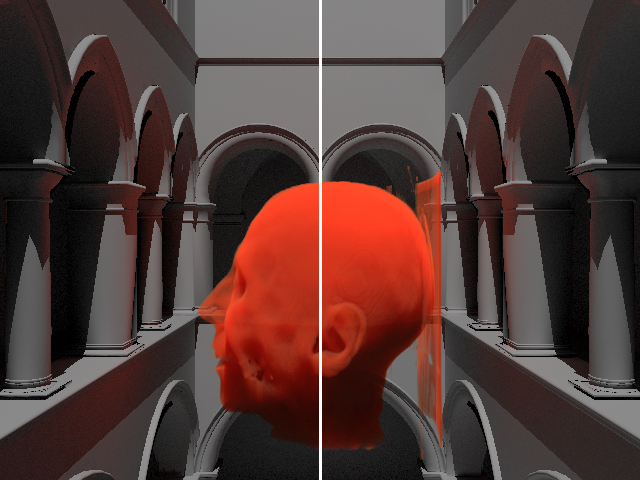
\includegraphics[width=90mm]{img/compare_head.png}
    \caption{CT Head scene comparison of the PCB extension (left) and traditional Monte Carlo results (right.)}
    \label{fig:compare2}
\end{figure}

\begin{figure}
\centering

\subfigure[]{%
    \label{fig:compare_first}
    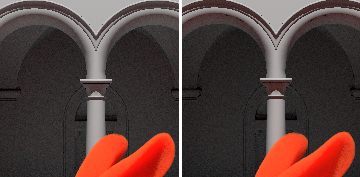
\includegraphics[width=0.65\linewidth]{img/compare1_corrected}
}\\
\subfigure[]{%
    \label{fig:compare_second}
    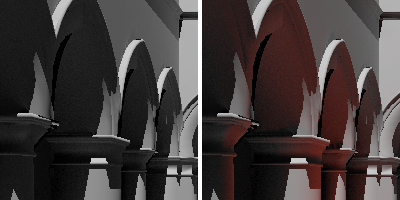
\includegraphics[width=0.65\linewidth]{img/compare_trad_corrected}
}

\caption{(a) Zoomed image showing traditional PCB (left) and PCB with extension (right.) and (b) Zoomed image showing PCB extension (left) and Monte Carlo (right.)}

\end{figure}

%------------------------------------------------------------%
\subsection{Data Comparison}

Table~\ref{tb:compare} shows render times, image differences and memory overhead for the CT scan datasets in the Sponza Atrium with varying sized volumes and for three different rendering methods: Monte Carlo without PCB, traditional PCB and finally our extended PCB algorithm.


\paragraph{Memory:}
When using traditional PCB, the real benefit to its surfel representation is shown in more complex scenes.  In the Sponza Atrium, the scene generated over 2.5 million surfels for a 60,000 triangle scene.  Adding volume data to the scene does not add an objectionable amount of data to the point cloud (see Table~\ref{tb:compare}), but for scenes with large volumes the costs could quickly add up without some form of multi-resolution light caching.  In this regard, adding yet another representation of the volumes may be expensive, but not prohibitively so.  Additionally, larger scenes would benefit from this representation, as the point cloud would be significantly simpler than the entire scene and can be moved to another system for out-of-core evaluation.

\setlength{\tabcolsep}{4pt}
\begin{table}
\begin{center}
\caption{Data for the Sponza Scene with the two different CT datasets.}
\label{tb:compare}
\begin{tabular}[b]{ | l | c | c | c | }
  \hline                       
  Scene: CT Bunny in Sponza & Render Time (s) & Image Delta & Memory Overhead \\

  \hline
  \multicolumn{4}{|c|}{$64^3$ resolution volume} \\     
  \hline            

  Monte Carlo w/o PCB & 3229 sec & NONE & NONE \\
  Traditional PCB & 348 sec & 5.8\% & 466.3 MB (4.780\%) \\
  Extended PCB & 433 sec & 2.1\% & 466.7 MB (4.786\%)  \\

  \hline
  \multicolumn{4}{|c|}{$128^3$ resolution volume} \\     
  \hline            
             
  Monte Carlo w/o PCB & 3297 sec & NONE & NONE \\
  Traditional PCB & 348 sec & 5.6\% & 466.3 MB (4.780\%) \\
  Extended PCB & 402 sec & 2.4\% & 467.5 MB (4.783\%)  \\

  \hline
  \multicolumn{4}{|c|}{$512^3$ resolution volume} \\     
  \hline            
             
  Monte Carlo w/o PCB & 3674 sec & NONE & NONE \\
  Traditional PCB & 348 sec & 9.6\% & 466.3 MB (4.780\%) \\
  Extended PCB & 417 sec & 3.8\% & 466.4 MB (4.785\%)  \\
  \hline  
  \hline  
             
%  \smallskip
  Scene:CT head in Sponza & Render Time (s) & Image Delta & Memory Overhead \\

  \hline
  \multicolumn{4}{|c|}{$64^3$ resolution volume} \\     
  \hline            

  Monte Carlo w/o PCB & 10150 sec & NONE & NONE \\
  Traditional PCB & 348 sec & 14.2\% & 466.3 MB (4.780\%) \\
  Extended PCB & 756 sec & 3.7\% & 468.0 MB (4.800\%)  \\

  \hline
  \multicolumn{4}{|c|}{$128^3$ resolution volume} \\     
  \hline            
             
  Monte Carlo w/o PCB & 15811 sec & NONE & NONE \\
  Traditional PCB & 348 sec & 14.4\% & 466.3 MB (4.780\%) \\
  Extended PCB & 755 sec & 4.2\% & 467.3 MB (4.790\%)  \\

  \hline
  \multicolumn{4}{|c|}{$256^3$ resolution volume} \\     
  \hline            
             
  Monte Carlo w/o PCB & 31373 sec & NONE & NONE \\
  Traditional PCB & 348 sec & 14.2\% & 466.3 MB (4.780\%) \\
  Extended PCB & 864 sec & 4.3\% & 467.1 MB (4.790\%)  \\
  \hline  
\end{tabular}
\end{center}
\end{table}
\setlength{\tabcolsep}{1.4pt}

%----------------------------------%
\paragraph{Speed:}
Even without volume integration, Monte Carlo integration without a lighting representation like PCB is prohibitively slow for even the simplest scenes.  Adding a point cloud representation gave us an impressive speedup.  That speedup was compounded even more when volume scattering was added into the tests, showing a speedup upwards of 36 times that of the Monte Carlo renders.  Compared to traditional PCB runs, we found the increase in overall runtime to be well worth the improvements to the renders we achieved. Even on sparse octrees without volumes, our \textit{front to back} octree traversal operates at an efficiency of $O\log{n}$ for each node traversal while skipping nodes occluded by surfels, leading to an average performance increase of over 18\%.

%----------------------------------%
\paragraph{Image Quality:}
To objectively compare rendering results, we used a perceptual image difference program called pdiff to identify how close any two renders matched.  The results, which ranged from 2.1\% and 4.3\%, are shown in Table \ref{tb:compare}.  Figure~\ref{fig:compare_first} compares the non-PCB Monte Carlo image with that of the traditional PCB renders, showing the clear lack of proper in-/out-scattering.  With the extended algorithm, however, the results are comparable.

\subsection{Conclusion}

We have presented an extension to the PCB algorithm by~\cite{christensen:2008} which handles both scatter-in and scatter-out contributions.  The addition of the lvoxel paradigm to the already successful point-based color bleeding algorithm is shown to be a cost effective method of approximating and evaluating complex scatter functions based on participating media.  We obtained render speeds up to 36 times faster than that of pure Monte Carlo renders with a memory overhead between 2 to 5 MB with an image difference of less than 5\% across all tests.

%==============================================================================%
\subsection{Future Work}

In our tests, we focused on isotropic phase functions in our volumes, while many volumes could have unique scatter functions.  We could simulate more complex surface scattering functions by creating spherical harmonic representations of the radiance at any specific point in the volume.  %Our current implementation supports such an approach, but remains untested.  
Another fruitful addition to our current method would be including rougher estimations, usually in the form of a series of spherical harmonic coefficients, at higher levels in the octree, to be evaluated depending on that node's solid angle to a sample point (often present in traditional PCB algorithms). Finally, as mentioned by Christensen~\cite{christensen:2008}, surfels can be modified to ``gather'' light recursively from their position in the point cloud, allowing for simulated multi-bounce lighting.  This would require only a small change to the current algorithm, and would apply to volumes as well to allow very realistic scatter approximations in participating media.

 %Due to time constraints, we did not implement full multi-resolution representations of each node.  Including LVoxel data in that representation would be a trivial process.

\section*{Acknowledgements}
A special thanks to Patrick Kelly from DreamWorks Animations for his consistent help and support.  Our brainstorming sessions were invaluable, and always left me full of new ideas as well as helping me hone the subject for this project.

\begin{figure}
    \centering
   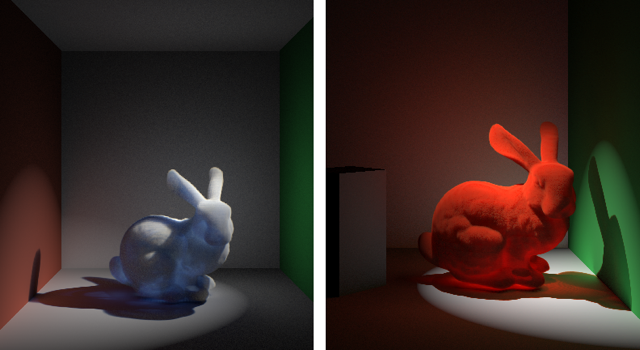
\includegraphics[width=120mm]{img/Two_Bunnies.png}
    \caption{On the left is  an image exemplifying clear out-scattering from Stanford bunny volume.  The right shows an image exemplifying clear color bleeding next to the red wall in the bunny's shadow and correct transmittance through the bunny's hollow form.}
\end{figure}

\bibliographystyle{pbcbex}
\bibliography{pbcbex}


%\begin{figure}[h!]
%    \centering
 %   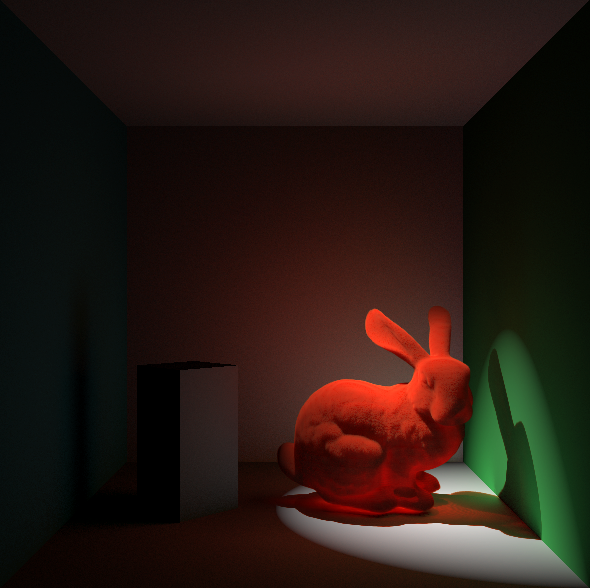
\includegraphics[width=80mm]{img/ketchup_good_corrected.png}
   % \caption{Image exemplifying clear out-scattering from Stanford bunny volume.}
%\end{figure}

%\begin{figure}[h!]
%    \centering
 %   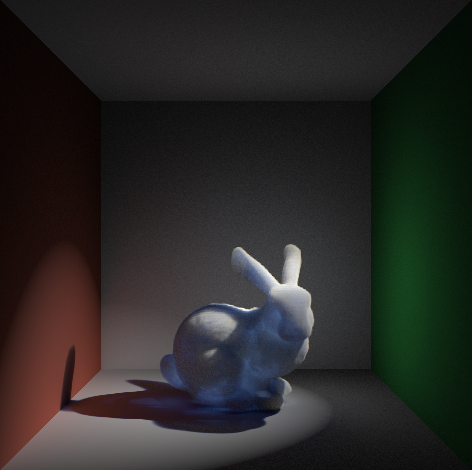
\includegraphics[width=80mm]{img/bunny_spot/spot_right_new.png}
%    \caption{Image exemplifying clear color bleeding next to the red wall in the bunny's shadow and correct transmittance through the bunny's hollow form.}
%\end{figure}

%\begin{figure}[h!]
   % \centering
  %  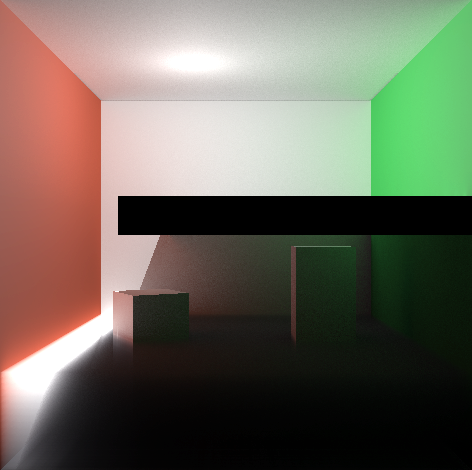
\includegraphics[width=80mm]{img/one_side_corrected.png}
 %   \caption{The black occluding geometry in the center stops all but the light to the left to enter below.  In and out scattering on the volume and walls is evident.}
%\end{figure}


\end{document}
